\section{Corpora and data audit}\label{sec:data}

\subsection{Corpora}
We use ten public corpora (Table~\ref{tab:corpora}). Seven share the veracity construct and form the main transfer matrix: two article corpora, ISOT \citep{ahmed2017isot,ahmed2018isot} and WELFake \citep{verma2021welfake}; two headline corpora from FakeNewsNet, PolitiFact and GossipCop \citep{shu2020fakenewsnet}, for which the public release contains titles and URLs; the claim corpus LIAR \citep{wang2017liar}, obtained through LIAR-PLUS \citep{alhindi2018liarplus}, binarised as \{pants-fire, false\} versus \{mostly-true, true\} with the two middle grades dropped; and the source tweets of Twitter15 and Twitter16 \citep{ma2017kernel}, using their false and true classes. Three further corpora extend the analysis to other constructs and to Bengali: the source tweets of PHEME rumour/non-rumour threads \citep{zubiaga2016phemernr,zubiaga2017context}; an English clickbait headline corpus \citep{chakraborty2016clickbait}; and BanglaBait \citep{mahtab2023banglabait}, \BBraw{} labelled Bengali news articles with machine-translated English titles. Labels differ in what they assert: LIAR rates individual claims, FakeNewsNet and Twitter15/16 rate a story through a fact-check, and ISOT and WELFake label articles largely by the outlet they came from. We keep these distinctions explicit and draw the strongest conclusions from four \emph{same-task pairs} that hold unit and construct fixed: ISOT$\leftrightarrow$WELFake (articles), PolitiFact$\leftrightarrow$GossipCop (headlines, politics vs.\ entertainment), Twitter15$\leftrightarrow$Twitter16 (tweets, two collection windows), and LIAR$\leftrightarrow$PolitiFact (claims vs.\ headlines from the same fact-checker). Every label is mapped to $1=$ fake, false, rumour or clickbait.

\paragraph{Provenance of the article files}
For the two article corpora we start from cleaned working copies made at an earlier stage of this project, and we reconstructed both from the original releases to document exactly how they were made (the script is in the repository). The ISOT release has \PvIsotRel{} articles in two files, one per class. Our copy keeps \PvIsotWork{} of them, all with their release labels: it lacks \PvIsotExact{} exact title-and-text duplicates and \PvIsotFurther{} further articles, \PvIsotFurtherTitle{} of which repeat the title of an article that was kept. The \PvIsotEmpty{} articles with an empty body keep their headline and are scored on it. The WELFake release (Zenodo, MD5 \texttt{\PvWelMD}) has \PvWelRel{} articles merged from four earlier collections, one of them a Reuters-based news set like ISOT's real class \citep{verma2021welfake,welfake2021data}. Our copy keeps \PvWelWork{}. Removing \PvWelExact{} exact duplicates, the \PvWelIsotText{} articles whose text also appears in the ISOT release and \PvWelIsotTitle{} more whose title does reproduces it up to \PvWelExtra{} articles, and no article of our copy lies outside this reconstruction. The overlap step matters: without it, about three in five deduplicated WELFake articles would be ISOT articles, and ISOT$\leftrightarrow$WELFake transfer would be inflated. After it, only \DupIW{} near-duplicates of ISOT remain, and those are excluded from every test (Section~\ref{sec:audit}). The repository includes loaders for both releases, so the whole pipeline, including this cleaning, can be rerun from the public files.

\begin{table}[t]
\centering
\caption{Corpora after harmonisation and deduplication. ``Exact'' and ``near'' count removed duplicates; ``conflict'' counts items removed because duplicates disagreed on the label; ``pos.'' is the share labelled fake, false, rumour or clickbait. For LIAR and Twitter15/16, ``raw'' counts the items in the binary view (LIAR: pants-fire/false vs.\ mostly-true/true; Twitter: false vs.\ true).}\label{tab:corpora}
\small
\begin{tabular}{@{}llllrrrrrr@{}}
\toprule
Corpus & Unit & Construct & Lang. & Raw & Exact & Near & Conflict & Final & Pos. \\
\midrule
ISOT & article & veracity & en & 38{,}833 & 0 & 79 & 0 & 38{,}749 & 0.46 \\
WELFake & article & veracity & en & 24{,}530 & 0 & 815 & 6 & 23{,}708 & 0.43 \\
PolitiFact & headline & veracity & en & 1{,}056 & 71 & 3 & 6 & 976 & 0.43 \\
GossipCop & headline & veracity & en & 22{,}140 & 1{,}174 & 26 & 380 & 20{,}560 & 0.23 \\
LIAR & claim & veracity & en & 8{,}090 & 21 & 11 & 3 & 8{,}055 & 0.44 \\
Twitter15 & tweet & veracity & en & 742 & 55 & 14 & 0 & 673 & 0.51 \\
Twitter16 & tweet & veracity & en & 412 & 51 & 3 & 0 & 358 & 0.46 \\
\midrule
PHEME & tweet & rumour & en & 5{,}802 & 124 & 98 & 25 & 5{,}555 & 0.34 \\
ClickbaitEN & headline & clickbait & en & 32{,}000 & 2 & 123 & 0 & 31{,}875 & 0.50 \\
BanglaBait & headline & clickbait & bn & 15{,}056 & 850 & 124 & 41 & 14{,}041 & 0.34 \\
\bottomrule
\end{tabular}
\end{table}


\subsection{Audit}\label{sec:audit}
\paragraph{Label direction}
Corpora disagree on which value denotes ``fake'', and nothing in a CSV file says which convention it follows. We therefore verify label direction with \emph{signature probes}: strings that only a reliable or only a fabricating outlet produces. Figure~\ref{fig:audit}a shows the result for the two article corpora. In ISOT, \ISOTreutersReal{} of the \ISOTreuters{} ``(Reuters)'' datelines carry label~0 and all \ISOTfiv{} texts with the fake-site template ``Featured image via'' carry label~1, so $1=$ fake. WELFake is more treacherous, because its documentation and its file disagree. The release record gives the legend $0=$ fake, $1=$ real \citep{welfake2021data}, but the file uses the opposite coding: all \WELrelNyt{} titles ending in ``- The New York Times'' carry label~0, all \WELrelFiv{} texts with ``Featured image via'' carry label~1, and \WELrelReu{} of the \WELrelReuN{} ``(Reuters)'' datelines carry label~0. The class sizes say the same. Label~1 holds \PvWelOne{} articles and label~0 \PvWelZero{}, which are the numbers of fake and real articles stated in the same record. Our working copy was made by following the legend: every label is the inverse of the release label, and a class-name column calls the inverted label~1 ``fake''. Our first pipeline trusted that column. Read that way, every ISOT$\leftrightarrow$WELFake score is inverted and ISOT$\to$WELFake looks like a below-chance collapse, while in-domain accuracy and macro-F1 are unaffected, which is why the error is easy to miss. The probes exposed it, and the loader now reverses the labels of the copy (or reads the release with the coding its file actually uses). A ranking metric below 0.5 on a same-task pair should be treated as a symptom to investigate before it is reported as a finding.

\begin{figure}[t]
\centering
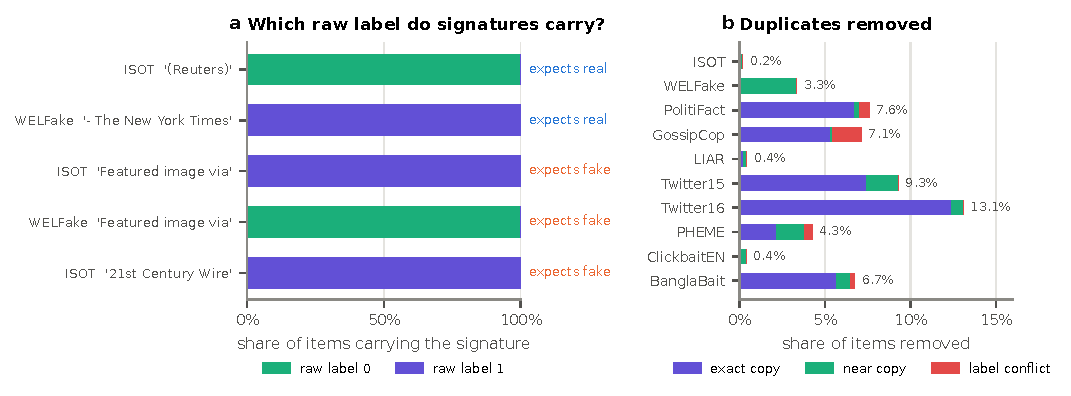
\includegraphics[width=\linewidth]{fig_audit}
\caption{Data audit. (a)~Label-direction probes: share of the items carrying an outlet signature that sit under raw label~0 or~1 (signatures found in at least 100 items). A reliable-outlet signature should sit under ``real'' and a fake-site signature under ``fake''. ISOT and the WELFake release both code $1=$ fake, although the WELFake record documents $0=$ fake; our working copy of WELFake, made by following that legend, has every label inverted. (b)~Share of items removed by deduplication: exact copies, near copies (MinHash, Jaccard $\geq0.8$) and items whose duplicates carried both labels.}\label{fig:audit}
\end{figure}

\paragraph{Duplicates}
Within each corpus we removed exact duplicates of the normalised text and then near-duplicates found by MinHash locality-sensitive hashing \citep{broder1997minhash} (128 permutations, Jaccard $\geq0.8$; word 3-grams for articles, character 5-grams otherwise). Groups whose members disagree on the label were dropped entirely. Table~\ref{tab:corpora} and Figure~\ref{fig:audit}b report the counts. Two corpora stand out. GossipCop contains \GCexact{} redundant exact copies of headlines, and a further \GCconflict{} rows whose headline appears under \emph{both} labels; BanglaBait contains \BBexact{} redundant exact copies of titles and, after deduplication, \BBfinal{} items. Even the cleaned WELFake copy still contained \WELnear{} near-duplicates.

\paragraph{Cross-corpus overlap}
Near-duplicates across corpora inflate transfer. ISOT and WELFake share only \DupIW{} near-duplicate articles, so the removal of shared articles from the WELFake copy worked. PHEME, however, shares \DupPT{} source tweets with Twitter15 and \DupPTs{} with Twitter16, because the corpora were collected around overlapping breaking-news events; Twitter15 and Twitter16 share \TwShared{} tweet identifiers, all labelled \emph{unverified}. Every transfer test excludes target items that are near-duplicates of the source corpus.
